\section{Desarrollo de software}

\subsection{Elección de arquitectura}
La decisión de software a usar depende del controlador a usar, poder de cálculo disponible, interfases de periféricos y funcionalidad deseada.

El controlador a usar es el ARM Cortex-A72 que sería comprado en el paquete comercial (\gls{soc}) conocido como \textit{Raspberry Pi 4B+}. El producto provee salidas para los siguientes usos

\begin{itemize}
    \item \glsxtrshort{uart}
    \item \glsxtrshort{spi}
    \item \glsxtrshort{i2c}
    \item \glsxtrshort{gpio}
\end{itemize}

La Raspberry Pi provee un entorno con Linux instalado que permite la programación con virtualmente cualquier lenguaje de programación en existencia. Dado estas condiciones, el lenguaje de programación elegido es \textbf{Go} (Golang) debido a los siguientes puntos

\begin{itemize}
    \item Seguro - Modelo de memoria Go, sistema de tipado fuerte\footnote{Hoy en día hay pocos lenguajes con sistemas de tipos fuertes. Contrario a la creencia popular, C y C++ ambos son tipados débilmente.}
    \item Simple - Claridad de sintaxis
    \item Concurrencia - Crear \glsplural{corrutina} es simple, paralelizar corrutinas es trivial
    \item Rendimiento - Superior a Python, Java y Matlab. Comparable a C. Esto también implica un menor consumo de energía
    \item Estable - \textit{The Go 1 promise} (La promesa Go 1)
    \item Comprobado -  Usado en sistemas de alto-riesgo/alta-complejidad (Kubernetes, Docker, Go-HEP)
    \item Portable - Todos los programas Go compilan a código nativo (código de máquina) para cualquier arquitectura y sistema operativo. Incluso se puede programar microcontroladores (TinyGo)
\end{itemize}


\newpage

\subsection{Flujo de control}
\begin{figure}[!htb]
    \centering
    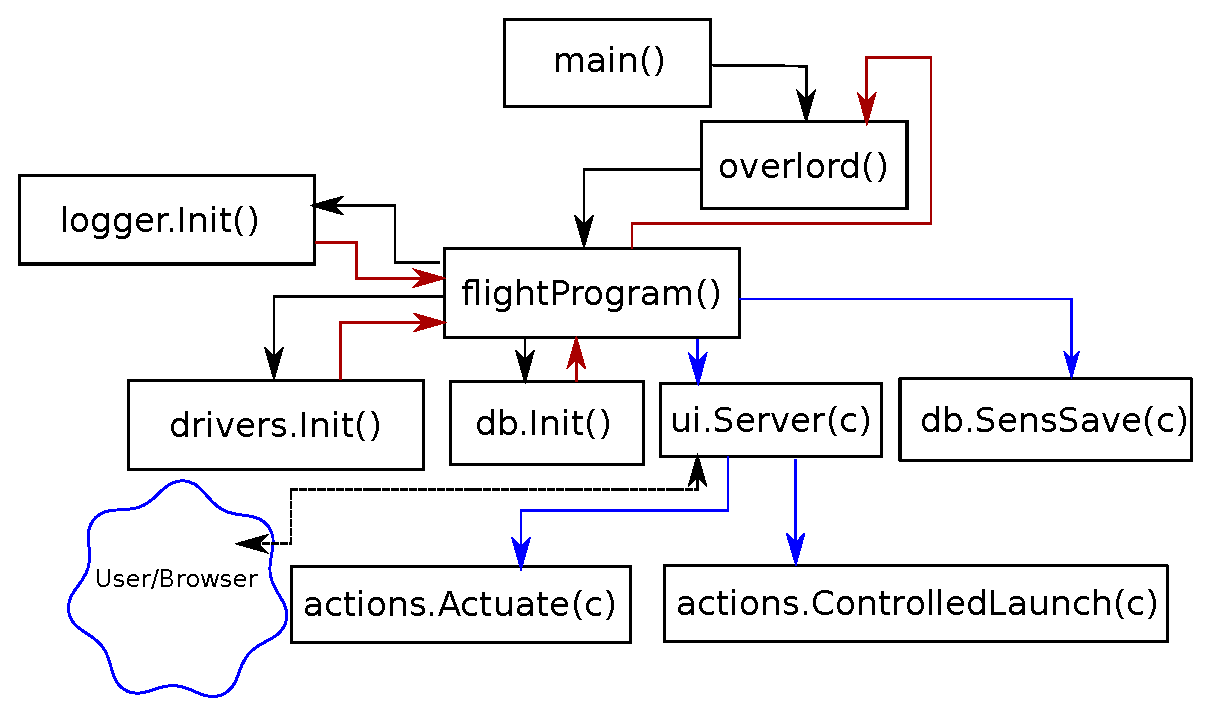
\includegraphics[width=0.7\textwidth]{fig/cfg_flightprogram.eps}
    \caption{Gráfico de flujo de control (CFG) del programa de vuelo. Las lineas de flujo azules son corrutinas independientes al programa principal. Las lineas negras son flujo del programa principal. Las lineas rojas son flujo del programa principal al encontrar un error.}
    \label{fig:flightProgram}
\end{figure}

Se ilustra el flujo de control a grandes rasgos usando un CFG en la figura \ref{fig:flightProgram}. El programa principal corre la rutina \texttt{overlord} que a su vez comanda \texttt{flightProgram} y espera que esta devuelva control a \texttt{overlord}. El propósito de \texttt{overlord} es guardar el estado del vehículo y ante una falla irrecuperable en \texttt{flightProgram}, terminar con todas las corrutinas generadas por \texttt{flightProgram} y sus afiliadas y a su vez reiniciar \texttt{flightProgram} nuevamente con el último estado antes de la falla.


\subsection{Interfaz con hardware}

Como se mencionó anteriormente, la computadora elegida tiene varios puertos que servirán como interfases con periféricos, entre ellos 

\begin{itemize}
    \item ADC (sensores)
    \item Generadores de PWM (para actuadores)
    \item Blinkenlights
\end{itemize}

Para la interacción del software con el hardware se usará la librería \href{https://periph.io}{periph.io}. Esta librería permite la interacción a través de los protocolos de comunicación de la Raspberry Pi. Los drivers para los periféricos fueron programados según la información dada en las datasheet.

\subsection{Implementación}

tbc

